\chapter{Results}
\label{results}

Different experiments have been done and stored. Below, a list of criteria for the creation of experiments is explained and a table with results for each experiment is presented.

\section{Control parameters}

The following is a list of parameters used to define different experiments.

\paragraph{Number of centers}

This parameter conditions the size of the real problem. It was made to test the model with smaller-size problems.

\paragraph{Patients' period size}

This parameter is a very important one. It groups appointments into patients (see \ref{sec:patients}) and it can do so in one of the following options (in minutes): "`No grouping"', 30, 60, 90, 120.

\paragraph{Solver}

Two solvers have been used: GUROBI and CBC. From the experiments, CBC was able to find feasible and reasonably good solutions for instances of less than 7 centers. GUROBI performed a lot better, as expected.

\paragraph{Solving time}

The following options of solving times were tried, in seconds: 25000, 40000.

\paragraph{Number of routes per vehicle}

The maximum number of routes that a vehicle can make. Values ranged between 2 and 4.

\paragraph{Other assumptions}

There was additional configuration that was tested during the development and construction of the model with small instances. It was not part of the experimentation process but does condition the quality of the solutions.

They are the following:

\begin{itemize}
	\item \textbf{Number of jobs per line}: 3, 5, 7, ..., 3 + 2 * (number of lines -1).
	\item \textbf{Total number of vehicles}: kept a the maximum.
	\item \textbf{Total number of lines}: kept at the maximum.
\end{itemize}

\section{Experiments}

Below are the results from the experiments that were run by doing changes in the parameters presented above.
Some of the parameter were not saved for some of the executions, like the solving time.


The best results were obtained when grouping patients into 60-minute blocks and 90-minute blocks. Using 2 routes per vehicle sometimes helped obtain a faster solution but not necessarily was better. Solving time was not highly relevant since the reduction on the gap was not significative.


The best gaps that were obtained got around 20\% and 40\%. None of the big instances was solved up to optimality.

\begin{center}
\begin{tabular}{c|c|c|c|c|c|c|c}
Experiment    & Solving  &  Period  &    Solver   &   Routes per &Centers &  Cost       &   GAP   \\
              & Time     &          &             &    vehicle   &        &             &   (\%)   \\ \hline
201705070923  & 25000         &  30      &    GUROBI   &   2          &  8     &  21132      &       \\ \hline
201705071205  &  5000         &  30      &    GUROBI   &   4          &  8     &  21432      &       \\ \hline
201705071948  & 25000         &  30      &    GUROBI   &   4          &  8     &  21432      &       \\ \hline
201705080316  & 25000         &  90      &    GUROBI   &   4          &  8     &  18438   &  23.1    \\ \hline
201705090800  & 40000         &  30      &    GUROBI   &   4          &  8     &  18738   &  36.1     \\ \hline
201705212256  & 3000          &  60      &    CBC      &   4          &  4     &  11359   &       \\ \hline
201705220557  & 25000         &  60      &    CBC      &   4          &  8     &  30617    &  208    \\ \hline
201705230608  & 25000         &  60      &    GUROBI   &   2          &  8     &  18482    &  31.5    \\ \hline
201705021351  &               &  30      &    GUROBI   &   2          &  3     &  12478   &       \\ \hline
201705021437  &               &  60      &    GUROBI   &   2          &  3     &  12478   &       \\ \hline
201705021554  &               & 120      &    GUROBI   &   2          &  8     &  18911   &       \\ \hline
201705070048    &             & None     &  GUROBI      &   4           &   8   &   30208 &      \\ \hline
201705070150    &               &   60      &   GUROBI  &   4           &   8   &   21732    &          \\ \hline
201705081624   & 25000         &   120      &   GUROBI  &   4           &   8   &   20538    &  32.5 \\ \hline
201705091923   & 40000         &   None      &   GUROBI  &   4           &   8   &   19974    &  50.5 \\ \hline
    \end{tabular}
\end{center}

\subsection{Solution}

As an example of how the solution is interpreted, a graph has been produced in figure \ref{fig:solution} to show the production and routing in one of the cases. The case being shown is "`201705230608"'.

The graphs assumes that time = 0 equals 7:00 AM in the morning.

In the first rows (production lines), identified with the name "`Line X"' the following is true:

\begin{itemize}
	\item colors mark the job type.
	\item tasks mark production jobs.
\end{itemize}

In the following rows (vehicles), identified with the name "`Vehicle X"' the following is true:

\begin{itemize}
	\item each color is the center from where vehicle exits (red is the production node).
	\item each task is the duration of the trip of the vehicle.
\end{itemize}

\begin{figure}
	\centering
		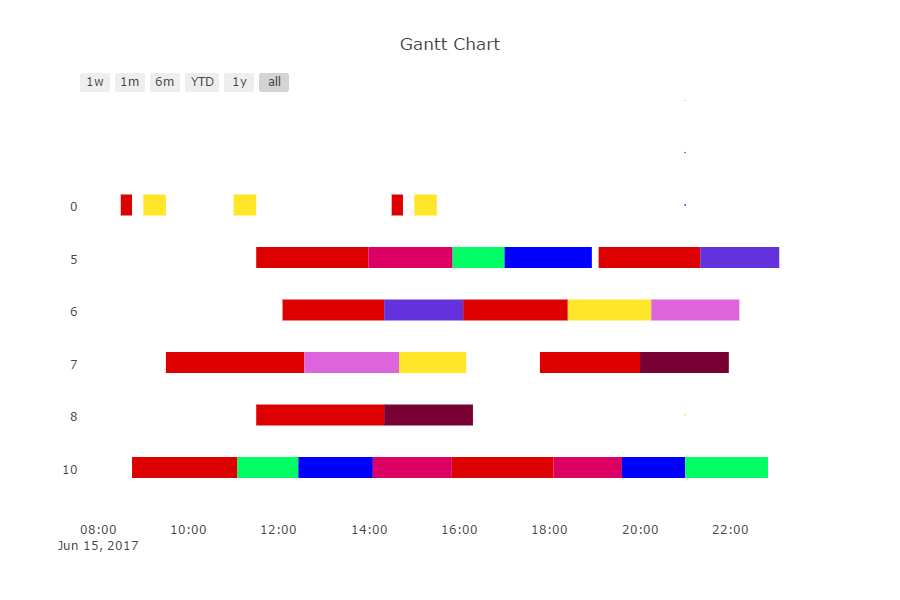
\includegraphics[width=\textwidth]{imagenes/production_and_routes.png}
	\caption{Production and routing}
	\label{fig:solution}
\end{figure}
